\documentclass[10pt]{article}

\usepackage[letterpaper,margin=0.82in]{geometry}
\usepackage{amsmath,amssymb}
\usepackage{booktabs}
\usepackage{graphicx}
\usepackage{microtype}
\usepackage[numbers,sort&compress]{natbib}
\usepackage{enumitem}
\usepackage[table,xcdraw]{xcolor}
\usepackage{hyperref}
\usepackage{caption}
\usepackage{subcaption}
\usepackage{array}
\usepackage{tabularx}
\usepackage{longtable}

\definecolor{keystoneblue}{HTML}{163B64}
\definecolor{statusgray}{HTML}{F1F3F5}
\hypersetup{
  colorlinks=true,
  linkcolor=keystoneblue,
  citecolor=keystoneblue,
  urlcolor=keystoneblue,
  pdftitle={KEYSTONE: Auditable Dispute-Key Availability for Encrypted AI Rollups},
  pdfauthor={Zubaer Mahmood Zubraj},
  pdfsubject={External PhD Reviewer Manuscript},
  pdfkeywords={dispute-key availability, threshold decryption, encrypted rollups, readiness audit, selective withholding}
}

\setlist{nosep,leftmargin=*}
\captionsetup{font=small,labelfont=bf}
\newcommand{\DKA}{\mathrm{DKA}}
\newcommand{\CA}{\mathrm{CA}}
\newcommand{\AKR}{\mathrm{AKR}}
\newcommand{\DDL}{\mathrm{DDL}}
\newcommand{\PAC}{\mathrm{PAC}}
\newcommand{\KeystoneDraftTableNotice}{\textbf{DRAFT / PRE-AUTHORIZATION:} This table is a preauthorization artifact and \textit{not} confirmatory or independent evidence.}

\title{\textbf{KEYSTONE: Auditable Dispute-Key Availability for Encrypted AI Rollups}}
\author{
  Zubaer Mahmood Zubraj\\
  \small Department of Computer Science, East Delta University\\
  \small Chittagong, Bangladesh\\
  \small \href{mailto:zmzubraj@gmail.com}{zmzubraj@gmail.com}
}
\date{External PhD Review Draft --- 30 August 2026}

\begin{document}
\maketitle

\begin{abstract}
Encrypted optimistic rollups may preserve the availability of ciphertext and execution receipts while failing when a dispute requires timely authorized decryption. This paper studies that gap as \emph{dispute-key availability} (DKA): the conditional ability of an authorized verifier to obtain at least a threshold number of valid decryption contributions before a dispute deadline, while preserving confidentiality before authorization. KEYSTONE is a non-production cryptographic-systems design that combines established threshold-KEM and verifiable partial-decryption components with an unpredictable canary audit, a public request/deadline transcript, and failure-domain-aware sampling. For a committee of $n$ custodians, threshold $t$, audit sample size $s$, and acceptance threshold $q$, we derive a hypergeometric false-accept expression for static catastrophic states. At the frozen baseline $n=32$, $t=22$, and $s=q=8$, the worst-case catastrophic false-accept probability is $\binom{21}{8}/\binom{32}{8}=0.0193463$, corresponding to a detection probability of $0.980654$. An internal exploratory selective-withholding sweep also provides a constructive limitation: eleven custodians can answer every non-production audit while refusing a target dispute, leaving only twenty-one responses and preventing threshold reconstruction. This result shows why an audit is evidence of present sampled serviceability, not a proof of future cooperation. The contribution is therefore a property separation, an integration design, and a bounded analysis---not a new threshold-encryption primitive or a claim of production security. Novelty relative to the strongest recovered predecessor set remains under independent review, and all simulation and prototype outputs are explicitly preliminary rather than confirmatory.
\end{abstract}

\noindent\textbf{Keywords:} dispute-key availability; threshold decryption; encrypted rollups; readiness sampling; selective withholding; accountability.

\vspace{0.6em}
\noindent\textbf{Review status.} This is an external scientific-review manuscript. The analytic result is model-bounded; the prototype and simulation outputs are internal and preliminary. Novelty is unresolved, feasibility has not been promoted to an authorized confirmatory study, and this document must not be treated as a submission-ready or production-security claim.

\section{Introduction}

Private or encrypted optimistic execution introduces an operational dependency that public data-availability mechanisms do not remove. A ciphertext can remain retrievable while the threshold service needed to open its record key is unavailable, late, invalid, or selectively uncooperative. In an optimistic dispute, that difference is decisive: the system must recover enough valid contributions after authorization and before a deadline, not merely prove that encrypted bytes exist.

KEYSTONE studies this distinction in the setting of encrypted AI-rollup disputes. The system keeps each inference record encrypted under a fresh symmetric key and wraps that key under an epoch threshold public key. A routine audit samples custodians using post-commit randomness and asks each sampled custodian to operate on a canonical, non-production group element. A valid response demonstrates current access to the custodian's epoch share and the ability to perform the required partial-decryption operation. An authorized dispute instead requests partial decryptions of the target record's threshold-KEM component. These two paths share cryptographic machinery but measure different behavior.

The central research question is:

\begin{quote}
How can an encrypted AI rollup obtain publicly auditable, non-revealing evidence that at least $t$ valid threshold-decryption contributions are currently serviceable for an authorized dispute before deadline $\Delta$, under explicit churn and correlated-failure assumptions, without releasing a production key or plaintext before authorization?
\end{quote}

The proposed contribution is deliberately narrow:

\begin{enumerate}
  \item a decomposition that separates ciphertext availability, valid-share registration, audit-time readiness, authorized decryptability, and dispute deadline liveness;
  \item a non-production canary audit constructed from established threshold-decryption and equality-of-discrete-log proof techniques;
  \item a closed-form false-accept bound for a static catastrophic readiness state, with explicit limits on repeated-audit inference; and
  \item an executable internal prototype and adversarial simulator that expose both useful evidence and a selective-withholding failure boundary.
\end{enumerate}

The paper does not claim a new threshold-encryption, VSS/PVSS, DLEQ, proactive-sharing, context-dependent-decryption, or bulletin-board primitive. It also does not claim that a successful audit proves unconditional future availability, adaptive selective-withholding resistance, or production security.

\section{Background and Related Work}

Data-availability sampling, including PeerDAS, concerns the retrievability of encoded public data and is therefore a contrast class rather than a solution to threshold-key serviceability \citep{eip7594}. Threshold encryption establishes that a ciphertext can be opened only with sufficiently many decryption contributions; classical and modern constructions supply the confidentiality and reconstruction substrate adopted here \citep{boneh2006threshold}. Verifiable secret sharing, proactive sharing, and dynamic proactive secret sharing address correct distribution, refresh, and changing committees, but do not by themselves measure whether a dispute service will meet a future deadline \citep{schoenmakers1999pvss,herzberg1995proactive,yurek2023dpss}.

Threshold-release systems already cover important parts of the design space. ETHTID studies deployable threshold information disclosure on Ethereum; Ferveo and BEAT-MEV apply threshold decryption to encrypted transaction ordering; vetKeys and time-lock encrypted storage address controlled blockchain disclosure; and context-dependent threshold decryption provides established context-isolation machinery \citep{stengele2021ethtid,bebel2022ferveo,bormet2025epochless,cerulli2023vetkeys,agarwal2025ttles,boneh2025context}. EigenAI provides adjacent encrypted/verifiable AI execution context rather than evidence for the present availability claim \citep{eigenai2026}. Accountability for threshold-decryption misbehavior and accountable liveness also constrain what public evidence can establish \citep{boneh2023accountability,lewis2025accountable}.

The bounded prior-art review therefore rejects broad primitive novelty. The surviving research hypothesis is whether the exact rollup-dispute framing---ciphertext/serviceability separation, pre-authorization canary exercise, explicit catastrophic false-accept analysis, correlated-failure qualification, and deadline evidence---constitutes a materially useful systems contribution. Absence of a single combined predecessor in the bounded search is not proof of novelty.

\section{System and Threat Model}

\subsection{Entities and records}

An epoch $E$ contains $n$ custodians and a threshold $t$. Custodian $i$ holds share $x_i$ and registers public share $Y_i=g^{x_i}$. A rollup worker encrypts record $r$ using a fresh symmetric key $K_r$ and an authenticated-encryption scheme. The worker wraps $K_r$ through a threshold Diffie--Hellman KEM under the epoch public key $PK_E$ and publishes the encrypted record and receipt to a data-availability layer. The settlement layer records the relevant commitment, policy, request, and deadline events.

The model includes the rollup worker, data-availability layer, custodian committee, randomness beacon, audit coordinator, policy/dispute contract, authorized verifier/combiner, and adjudication logic. The ledger supplies an ordered public clock. Cryptographic evidence for an invalid proof or equivocation is positive evidence; attributing a missed deadline to malicious behavior additionally requires a declared synchrony and delivery assumption.

\subsection{Readiness and security properties}

For request type $u\in\{\mathsf{audit},\mathsf{dispute}\}$, define
\[
\mathrm{Ready}_i(E,\tau,u,\Delta)=1
\]
iff custodian $i$ can access its valid current share, execute the required operation, generate a valid proof, and deliver its response by $\tau+\Delta$. Audit and dispute readiness are intentionally different: a target-aware custodian may answer a canary but refuse a particular dispute.

The relevant properties are:

\begin{itemize}
  \item \textbf{Ciphertext availability ($\CA$).} The encrypted record and receipt bytes are retrievable from the data-availability layer.
  \item \textbf{Valid-share registration.} The registered shares are consistent with one epoch threshold key according to the adopted DKG/VSS/PVSS layer.
  \item \textbf{Audit-time key-service readiness ($\AKR$).} At least $q$ members of a sampled set return valid, context-bound canary partial decryptions by the audit deadline.
  \item \textbf{Authorized decryptability.} Following valid authorization, an approved combiner obtains at least $t$ distinct valid partial decryptions of the target record component.
  \item \textbf{Dispute deadline liveness ($\DDL$).} Authorized decryptability completes by the dispute deadline.
  \item \textbf{Pre-authorization confidentiality ($\PAC$).} Before authorization, an adversary controlling fewer than $t$ current shares learns no information about the record key beyond leakage from the base encryption and metadata scheme.
\end{itemize}

Table~\ref{tab:properties} records each declared property, its role in the design, and the evidence boundary that applies to it at this review stage.

\begin{table}[h]
\centering
\caption{Declared readiness and security properties and their evidence boundaries. All rows are preauthorization design assertions; no row is confirmatory or independent evidence.}
\label{tab:properties}
\small
\begin{tabularx}{\textwidth}{>{\raggedright\arraybackslash}p{0.2\textwidth} X >{\raggedright\arraybackslash}p{0.3\textwidth} >{\raggedright\arraybackslash}p{0.25\textwidth}}
\toprule
Property & Definition in the manuscript & What it can support & Evidence stage\\
\midrule
$\CA$ & The encrypted record and receipt bytes are retrievable from the data-availability layer & Distinguishes ciphertext availability from dispute-key availability & DESIGN\_ONLY\\
Valid-share registration & Registered shares are consistent with one epoch threshold key according to the adopted DKG/VSS/PVSS layer & Establishes the trust anchor for later audit and dispute operations & DESIGN\_ONLY\\
$\AKR$ & At least $q$ members of a sampled set return valid, context-bound canary partial decryptions by the audit deadline & Audit-time readiness for the frozen local configuration & PREAUTHORIZATION\_INTERNAL\\
Authorized decryptability & Following valid authorization, an approved combiner obtains at least $t$ distinct valid partial decryptions of the target record component & Authorized dispute path feasibility under local prototype conditions & PREAUTHORIZATION\_INTERNAL\\
$\DDL$ & Authorized decryptability completes by the dispute deadline & Deadline-liveness performance & NOT\_EXECUTED\\
$\PAC$ & Before authorization, an adversary controlling fewer than $t$ current shares learns no information about the record key beyond leakage from the base encryption and metadata scheme & Confidentiality of the pre-authorization path & DESIGN\_ONLY\\
\bottomrule
\end{tabularx}
\end{table}

KEYSTONE defines $(\varepsilon,\Delta_d)$-DKA as the conditional property that, following valid authorization and under the stated readiness and network assumptions, the combiner obtains $t$ valid contributions by $\tau+\Delta_d$ with probability at least $1-\varepsilon$, while $\PAC$ holds before authorization. DKA is thus a deadline-bounded service property rather than an unconditional promise of future key availability.

\subsection{Adversaries and exclusions}

The model considers independent crash faults, provider/region/software-domain correlated outages, invalid or equivocal responses, changing compromise across epochs, selective withholding, beacon prediction or substitution, and unauthorized requests. Confidentiality assumes fewer than $t$ current shares are compromised. Production DKG/PVSS security, malicious authorized verifiers, arbitrary asynchronous partitions, and fully adaptive selective-withholding resistance remain out of scope.

\begin{figure*}[t]
  \centering
  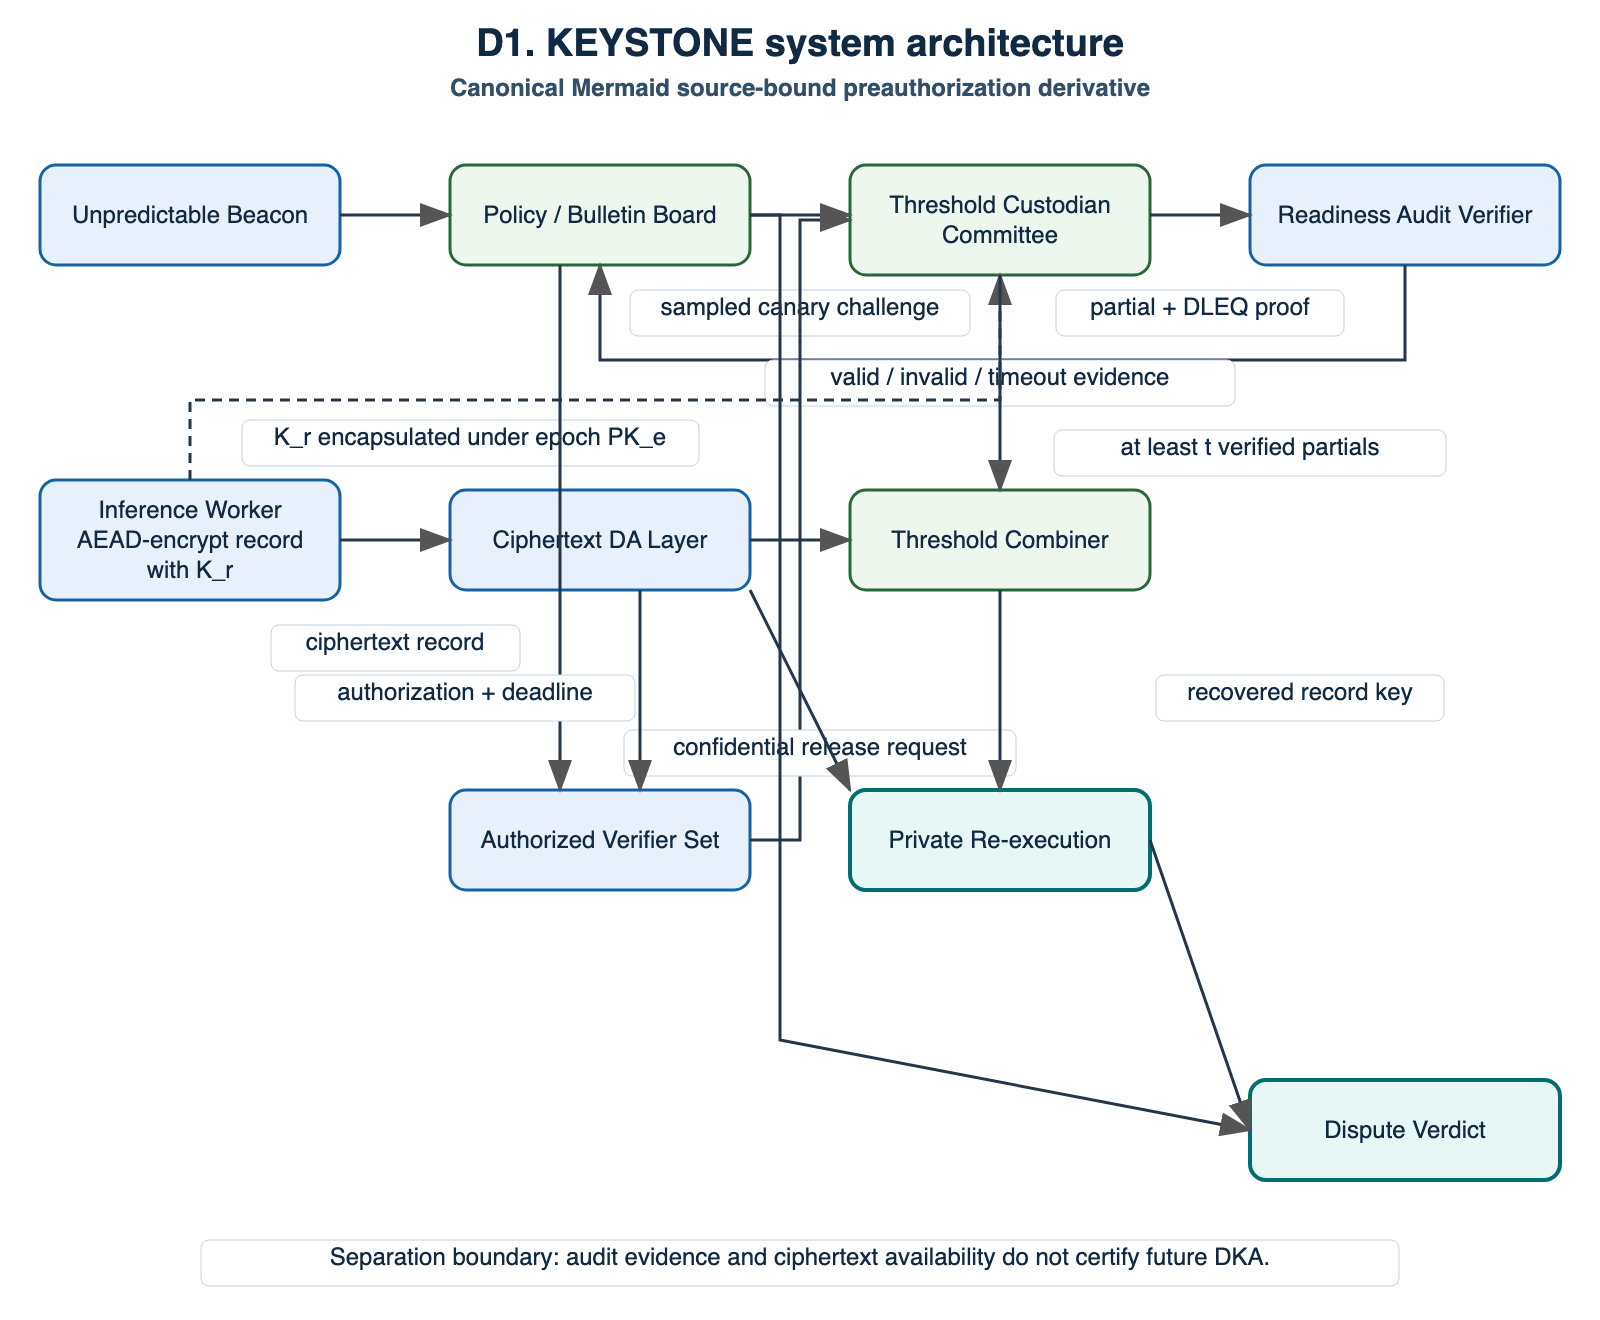
\includegraphics[width=0.94\textwidth]{../../diagrams/01_system_architecture.png}
  \caption{KEYSTONE architecture. Ciphertext publication, routine canary auditing, and authorized dispute-key release are separate paths. The diagram specifies the proposed interface; it does not establish that any component is externally deployed or production-secure.}
  \label{fig:architecture}
\end{figure*}

\section{KEYSTONE Protocol}

Figure~\ref{fig:architecture} summarizes the architecture. One threshold public key protects many record-specific data keys; custodians do not store one Shamir object per record.

\subsection{Epoch setup and record sealing}

The committee is formed subject to identity, stake, and failure-domain placement policy. A production system would use an authenticated DKG or PVSS; the current prototype uses a dealer and Feldman commitments only as a substitution boundary. The worker encrypts the record with AES-256-GCM under $K_r$, publishes threshold-KEM component $C_1=g^r$, derives $PK_E^r$, and uses the resulting KEM key to wrap $K_r$. The record envelope binds the epoch, record identifier, ciphertext, authenticated metadata, and data-availability pointer.

\subsection{Non-production readiness audit}

Before the beacon is known, the coordinator commits the epoch and audit slot. After finalization, the beacon determines a uniform or domain-stratified sample $S$ of size $s$. All parties derive the same challenge
\[
X=H_G(\texttt{KEYSTONE-CANARY}\parallel E\parallel \mathsf{slot}\parallel \mathsf{beacon}),
\]
where $H_G$ is domain separated and does not expose $\log_g X$. Sampled custodian $i$ returns $D_i=X^{x_i}$ and a Chaum--Pedersen equality-of-discrete-log proof binding $(g,Y_i,X,D_i)$ to the request context \citep{chaum1992dleq,rfc9380}. The verifier checks membership, identity, freshness, uniqueness, proof validity, and deadline. The audit accepts after $q$ valid responses. Because $X$ is a fresh non-production element, the audit exercises share access and partial-decryption capability without opening a production record.

\subsection{Authorized dispute release}

A dispute begins only after the policy contract accepts a challenge and binds the request to a record, epoch, authorized verifier set, and deadline. Each responding custodian verifies the authorization and returns a partial decryption of the record component $C_1$ through the approved channel, together with the permitted proof or commitment. The combiner verifies any $t$ distinct responses and interpolates in the exponent:
\[
\prod_{i\in I} (C_1^{x_i})^{\lambda_i}=C_1^{\sum_{i\in I}\lambda_i x_i}=C_1^x=PK_E^r.
\]
It then derives the KEM key, unwraps $K_r$, decrypts the record, and performs the authorized verification procedure. The public transcript can record valid, invalid, equivocal, stale, unauthorized, or missing responses while keeping plaintext release policy separate.

\section{Analysis}

\subsection{Static catastrophic false acceptance}

Let exactly $r<t$ custodians be audit-ready throughout one request. If $s$ custodians are sampled uniformly without replacement and acceptance requires at least $q$ valid responses, then
\begin{equation}
\Pr[\mathsf{accept}\mid r]
=\sum_{j=q}^{\min(s,r)}
\frac{\binom{r}{j}\binom{n-r}{s-j}}{\binom{n}{s}}.
\label{eq:hypergeom}
\end{equation}
This probability is monotone in $r$, so the worst catastrophic state is $r=t-1$. When $q=s$,
\begin{equation}
\varepsilon_a=\Pr[\mathsf{false\ accept}]\leq
\frac{\binom{t-1}{s}}{\binom{n}{s}}.
\label{eq:bound}
\end{equation}
For $n=32$, $t=22$, and $s=q=8$, Equation~(2) gives $\varepsilon_a=0.0193462822$ and detection probability $1-\varepsilon_a=0.9806537178$. These are exact values for the declared static model, not field-calibrated failure probabilities.

If the catastrophic ready set remains fixed and every sample is independently unpredictable, false acceptance in all $m$ audits is at most $\varepsilon_a^m$. This multiplication is invalid for a time-varying or adaptive adversary unless an explicit temporal model justifies it.

\subsection{Three non-implication witnesses}

The scientific core is not only the favorable bound. It also contains three constructive limitations:

\begin{enumerate}
  \item $\CA$ does not imply DKA: ciphertext remains available while only $t-1$ custodians are dispute-ready.
  \item $\AKR$ does not imply target-dispute success: selective custodians answer the canary but withhold the target response.
  \item A finite sequence of accepted audits does not imply unconditional future DKA: enough custodians may become unavailable after the last audit.
\end{enumerate}

These witnesses define what the audit can and cannot support. They prevent an operational health signal from being presented as a timeless availability proof.

\begin{figure*}[t]
  \centering
  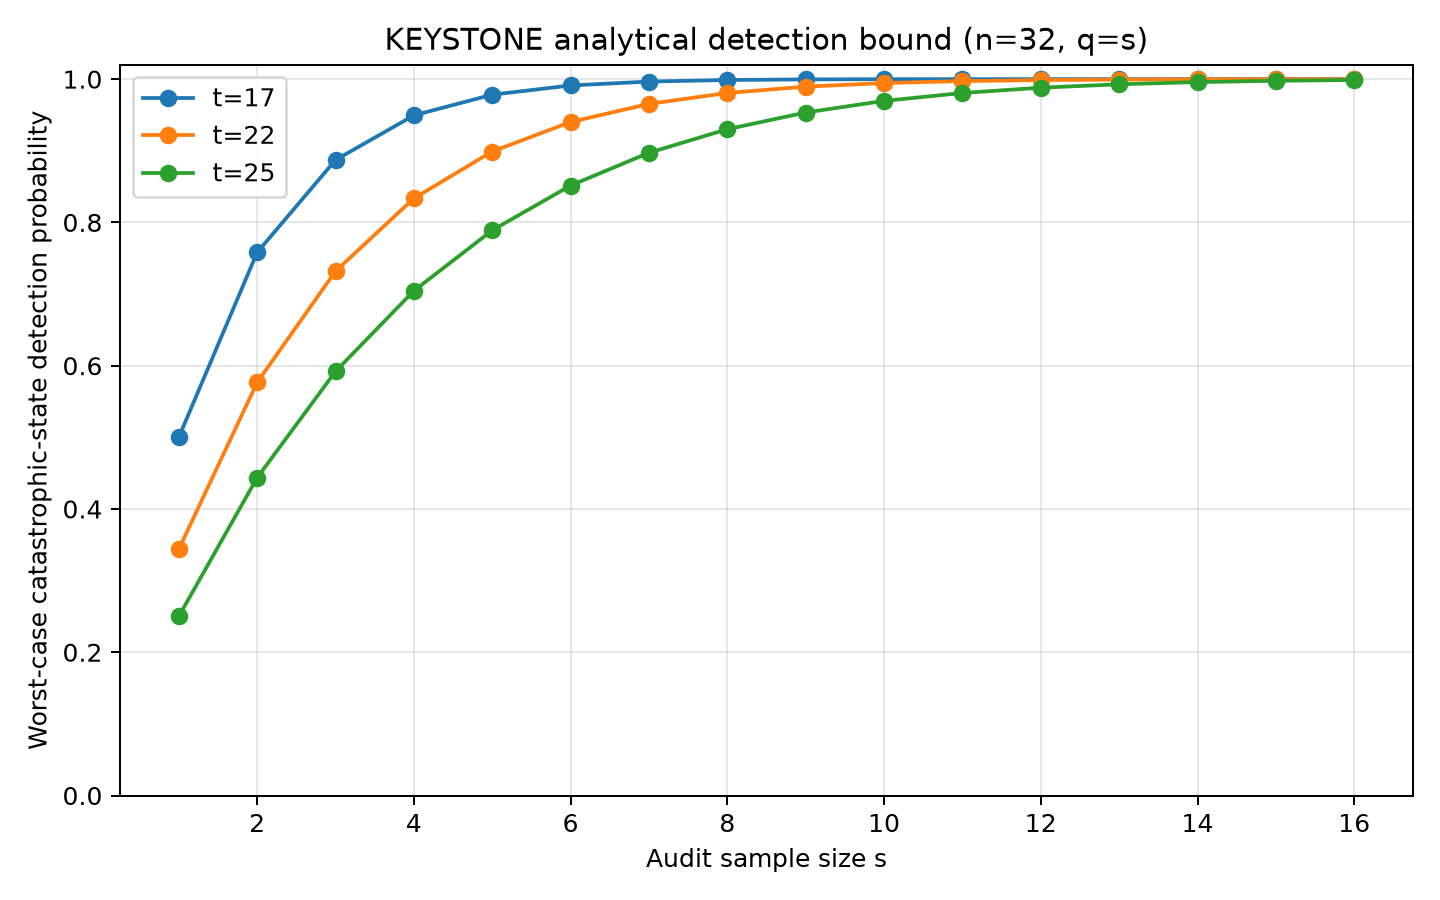
\includegraphics[width=0.72\textwidth]{../../prototype/results/figures/figure_1_theoretical_detection_bound.png}
  \caption{Exact static detection probability versus sample size for the frozen $n=32$ committee and several thresholds. The figure is deterministic under the stated static model and is not confirmatory or independently reproduced.}
  \label{fig:detection}
\end{figure*}

\begin{figure}[h]
  \centering
  \fbox{\parbox[c]{0.82\textwidth}{\centering\vspace{1.2em}
  \textbf{[BLOCKED: Figure 3 --- Dispute Success Probability versus Deadline]}\\[0.6em]
  RID-C003-DEADLINE-001 is in \textit{missing\_required\_evidence}. All four deadline environment profiles (control, latency, loss, crash) in\\
  \texttt{research-case/03-design/deadline-environment-profiles.csv} are $BLOCKED\_UNRESOLVED\_DESIGN$.\\
  \texttt{prototype/results/figures/figure\_3\_*.png/svg} are absent.\\
  \textit{This figure cannot be produced from existing repository evidence.}\vspace{1.2em}}}
  \caption{\textbf{Blocked ---} Dispute success probability as a function of deadline budget under latency, loss, and crash profiles. This figure is BLOCKED because all deadline environment profiles are unresolved distributed design and no corresponding deadline figure files exist.}
  \label{fig:deadline}
\end{figure}

\begin{figure*}[t]
  \centering
  \begin{subfigure}[t]{0.47\textwidth}
    \centering
    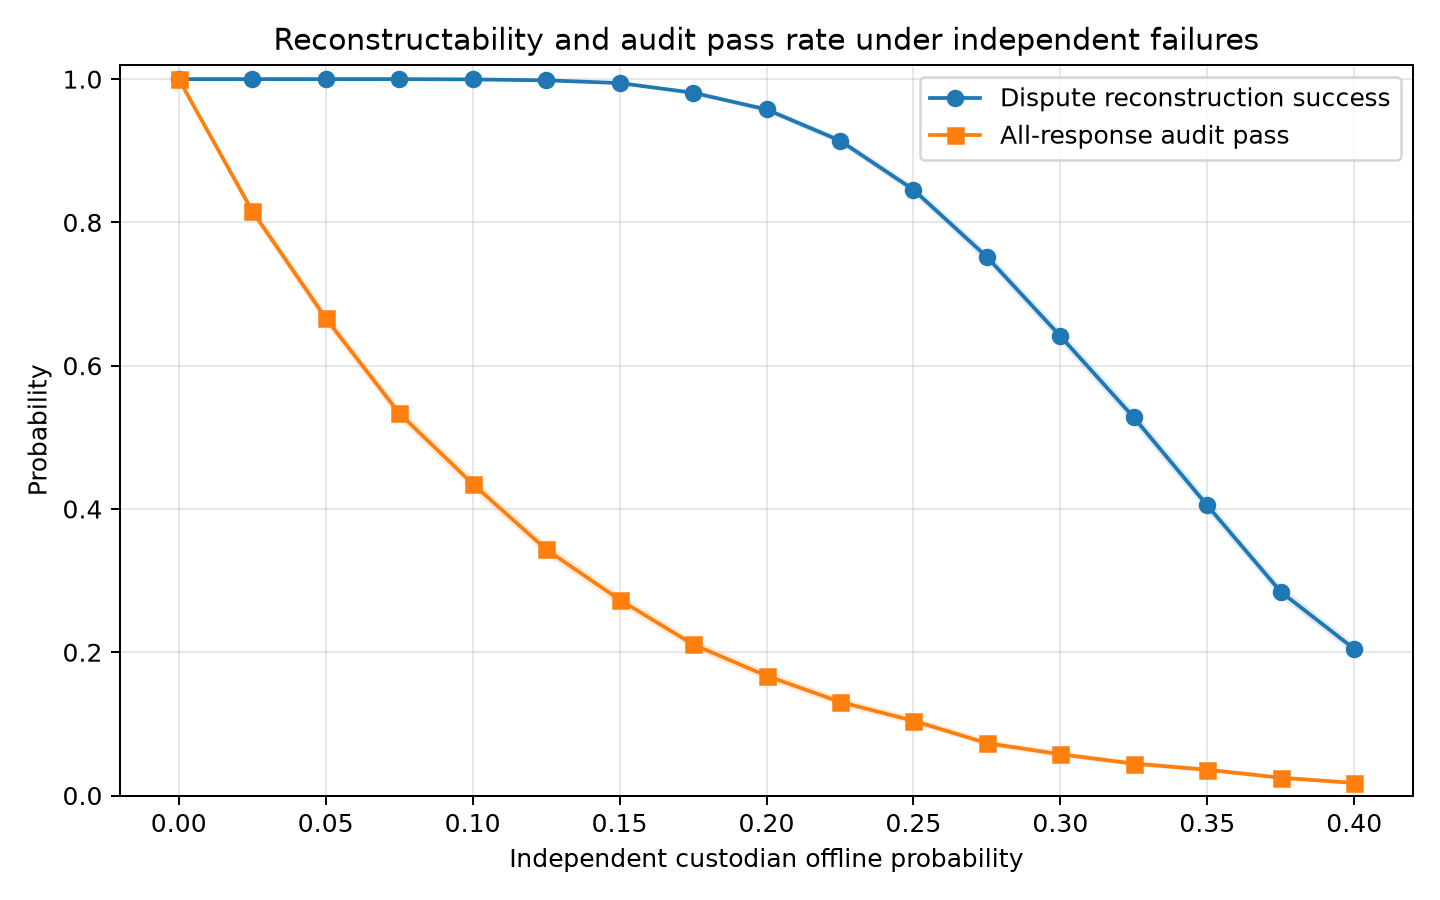
\includegraphics[width=\linewidth]{../../prototype/results/figures/figure_2_iid_failure_sweep.png}
    \caption{IID outage sweep at the frozen $n=32$, $t=22$, $s=8$, $q=8$ configuration with independent offline probabilities from 0 to 0.4.}
    \label{fig:iid}
  \end{subfigure}\hfill
  \begin{subfigure}[t]{0.47\textwidth}
    \centering
    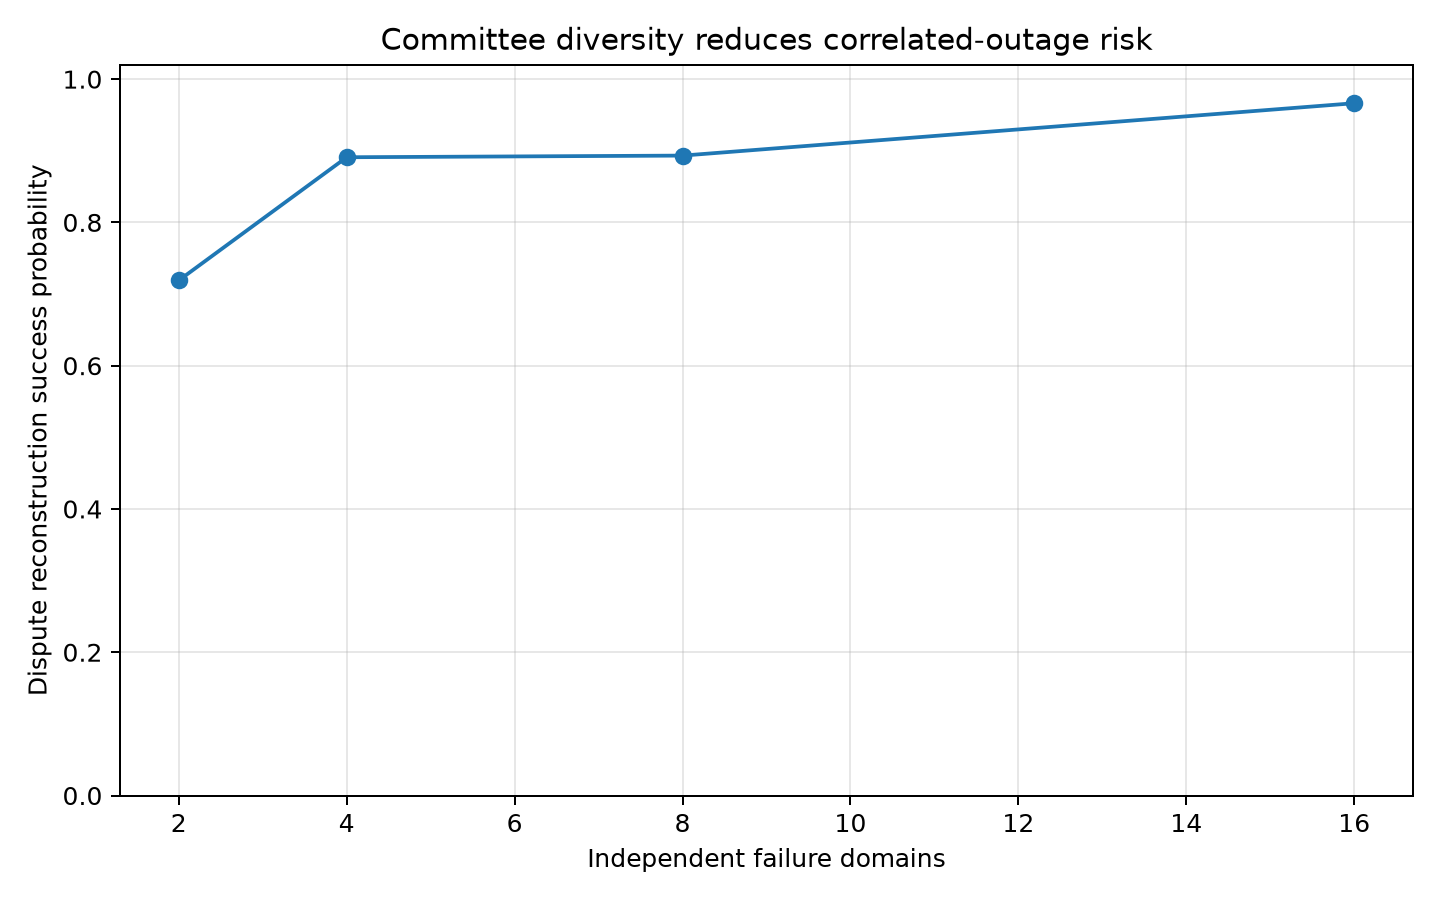
\includegraphics[width=\linewidth]{../../prototype/results/figures/figure_3_domain_diversity.png}
    \caption{Correlated domain outage sweep at the same frozen configuration. Correlated outages change response-count distributions differently than IID failures.}
    \label{fig:correlated}
  \end{subfigure}
  \caption{IID failure sweep (panel a) and correlated domain outage sweep (panel b). Both are internal seeded simulations with 4,000 trials per cell and are not confirmatory or independently reproduced.}
  \label{fig:failure-modes}
\end{figure*}

\begin{figure*}[t]
  \centering
  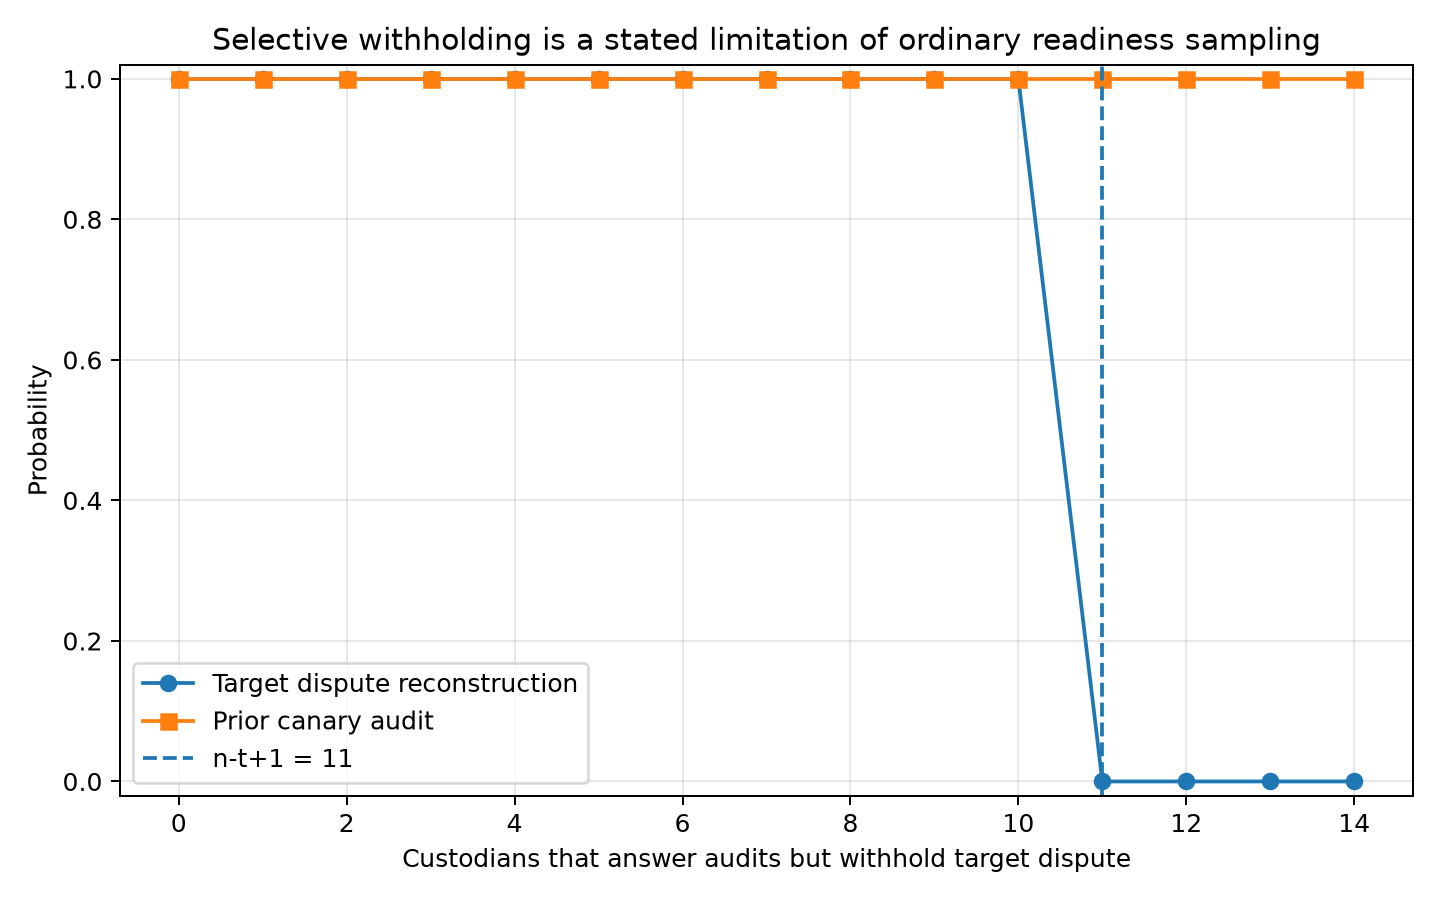
\includegraphics[width=0.72\textwidth]{../../prototype/results/figures/figure_4_selective_withholding_gap.png}
  \caption{Audit pass remains one while target reconstruction falls to zero at $w=n-t+1=11$ withholding custodians. Internal exploratory sweep with 4,000 trials per withholder count. Audit pass: $1.0$ [0.99904, 1.0]; reconstruction success: $0.0$ [0, 0.000959]. This figure is not confirmatory or independently reproduced.}
  \label{fig:withholding}
\end{figure*}

\section{Evaluation Design and Current Evidence}

\subsection{Evaluation questions}

The complete study asks whether measured false acceptance matches Equation~(1); how $(n,t,s,q)$ trades audit cost against detection; how correlated outages differ from IID failure; whether domain-stratified sampling changes catastrophic detection; what local cryptographic and ledger costs are incurred; and how strongly selective withholding separates audit success from dispute success. A later distributed experiment must separately measure whether $t$ verified responses arrive before $\Delta_d$ under declared latency, loss, and crash profiles.

\subsection{Evidence classes}

Table~\ref{tab:evidence} separates established observations from planned evidence. The distinction is essential because a clean local implementation does not validate novelty, external reproducibility, deadline performance, or production security.

\begin{table}[h]
\centering
\caption{Current evidence map and claim ceiling.}
\label{tab:evidence}
\small
\begin{tabularx}{\textwidth}{>{\raggedright\arraybackslash}p{0.21\textwidth} >{\raggedright\arraybackslash}p{0.22\textwidth} X >{\raggedright\arraybackslash}p{0.17\textwidth}}
\toprule
Evidence & Current status & What it can support & What it cannot support\\
\midrule
Static hypergeometric calculation & Deterministic analytic & Model-bounded false-accept and detection values & Temporal, adaptive, or field behavior\\
Selective-withholding sweep & Internal seeded simulation & Constructive audit/dispute separation within the simulator & Prevalence, external validity, or resistance\\
Threshold-KEM, DLEQ, serialization, and signature tests & Local engineering QA & Internal correctness and interface consistency & Cryptographic audit or production security\\
Solidity bulletin-board tests and gas receipts & Local test-body measurements & Contract-boundary behavior in the harness & Deployment cost or operational throughput\\
Distributed deadline study & Not executed & Nothing yet & Any deadline-liveness performance claim\\
Independent reproduction and external validation & Not completed & Nothing yet & Independent or field maturity\\
\bottomrule
\end{tabularx}
\end{table}

\subsection{Tables T2--T7: Evidence package}

Tables~\ref{tab:t2} and \ref{tab:t3} are rendered from empirical sources; Tables~\ref{tab:t4} and \ref{tab:t5} display preliminary Monte Carlo and resource measurements; Tables~\ref{tab:t6} and \ref{tab:t7} display robustness checks and unresolved risks. All tables bear the preauthorization notice.

\begin{table}[h]
\centering
\caption{\KeystoneDraftTableNotice\ \newline T2: Proposed design versus bounded baselines. KEYSTONE_FROZEN_DESIGN separates ciphertext availability from current authorized reconstructability, addressing C001/C003.}
\label{tab:t2}
\small
\begin{tabularx}{\textwidth}{@{}lXl@{}}
\toprule
Comparator & Design difference & Claim ceiling \\
\midrule
KEYSTONE\_FROZEN\_DESIGN & Separates ciphertext availability from current authorized reconstructability & ASSERTED\_ONLY\\
CIPHERTEXT\_DA & Does not by itself establish threshold-key serviceability & NOT\_MEASURED\\
GENERIC\_THRESHOLD\_RELEASE & Prior art already occupies generic threshold release; KEYSTONE comparison is narrower & NOT\_MEASURED\\
UNIFORM\_CANARY\_SAMPLING & Reference policy for planned stratified and correlated comparisons & ASSERTED\_ONLY\\
\bottomrule
\end{tabularx}
\end{table}

\begin{table}[h]
\centering
\caption{\KeystoneDraftTableNotice\ \newline T3: Experimental conditions and frozen profile. RID-C003-DEADLINE-001 remains BLOCKED/unresolved.}
\label{tab:t3}
\small
\begin{tabularx}{\textwidth}{@{}p{0.16\linewidth}p{0.16\linewidth}p{0.32\linewidth}p{0.25\linewidth}@{}}
\toprule
Environment & CPU/Machine & Failure mode & Execution status \\
\midrule
LOCAL\_SIMULATION & 4 domains, 8 custodians each & IID offline probability 0 to 0.4 & Executed \\
DOMAIN\_OUTAGE\_20PCT\_STRATIFIED & 4 domains, 20\% offline per domain, stratified sampling & Correlated domain failure & Executed \\
RID-C003-DEADLINE-001 & DISTRIBUTED\_MULTI\_PROCESS\_OR\_MULTI\_MACHINE\+\_\+PROFILE\_MISSING & Distributed latency/loss/crash conditions & \textbf{NOT EXECUTED -- BLOCKED} \\
\bottomrule
\end{tabularx}
\end{table}

\begin{table}[h]
\centering
\caption[\texorpdfstring{T4: Preliminary Monte Carlo outcomes}{T4: Preliminary Monte Carlo outcomes}]{\KeystoneDraftTableNotice\ \newline T4: Preliminary Monte Carlo outcomes with 95\% Wilson score intervals. Catastrophic detection is conditioned on the reported number of catastrophic trials.}
\label{tab:t4}
\small
\begin{tabular}{lrrrr}
\toprule
Scenario & Trials & Reconstruction & Audit pass & Detection (conditional $n$) \\
\midrule
IID 10\%, uniform & 20,000 & 0.99975 [0.99941, 0.99989] & 0.42905 [0.42220, 0.43592] & 1.00000 [0.56552, 1.00000] (5) \\
Domain outage 20\%, uniform & 20,000 & 0.81360 [0.80814, 0.81894] & 0.37125 [0.36458, 0.37797] & 0.99759 [0.99542, 0.99873] (3,728) \\
Domain outage 20\%, stratified & 20,000 & 0.81430 [0.80885, 0.81963] & 0.33895 [0.33242, 0.34554] & 1.00000 [0.99897, 1.00000] (3,714) \\
11 selective withholders & 20,000 & 0.00000 [0.00000, 0.00019] & 1.00000 [0.99981, 1.00000] & 0.00000 [0.00000, 0.00019] (20,000) \\
\bottomrule
\end{tabular}
\end{table}

\begin{table}[h]
\centering
\caption[\texorpdfstring{T5: Real-world feasibility and resource boundary}{T5: Real-world feasibility and resource boundary}]{\KeystoneDraftTableNotice\ \newline T5: Local cryptographic microbenchmarks and Foundry test-body gas measurements. All timing measurements use local repeats; gas excludes setup overhead and small harness artifacts.}
\label{tab:t5}
\small
\begin{tabular}{lr}
\toprule
Operation & Value \\
\midrule
Keygen, n=16 & 16.9 ms \\
Keygen, n=32 & 67.7 ms \\
Keygen, n=64 & 310.8 ms \\
Open, n=16 & 8.6 ms \\
Open, n=32 & 17.4 ms \\
Open, n=64 & 34.7 ms \\
\addlinespace
register\_epoch & 223,629 gas \\
open\_audit & 125,107 gas \\
submit\_audit\_response & 57,882 gas \\
mark\_invalid\_response & 27,704 gas \\
record\_equivocation & 51,710 gas \\
finalize\_audit & 29,142 gas \\
open\_dispute & 144,149 gas \\
cancel\_request & 5,709 gas \\
\bottomrule
\end{tabular}
\end{table}

\begin{table}[h]
\centering
\caption[\texorpdfstring{T6: Robustness and boundary conditions (excerpt)}{T6: Robustness and boundary conditions (excerpt)}]{\KeystoneDraftTableNotice\ \newline T6: Robustness and boundary-condition checks (excerpt). Full table has 34 records: 17 IID outage cells, 9 matched-seed sampling comparisons, 1 exact stratified validation, and 4 temporal-Markov cells.}
\label{tab:t6}
\small
\begin{tabular}{lcccl}
\toprule
Check & Offline prob. & Reconstruction & Audit pass & Boundary \\
\midrule
ROB-IID-0000 & 0.000 & 1.000 & 1.000 & Baseline \\
ROB-IID-0100 & 0.100 & 0.9996 & 0.435 & Detection ceiling \\
ROB-IID-0200 & 0.200 & 0.9577 & 0.167 & Degraded regime \\
ROB-IID-0300 & 0.300 & 0.6413 & 0.058 & Severe outage \\
ROB-IID-0400 & 0.400 & 0.2047 & 0.018 & Near-total failure \\
ROB-SAMPLING-08-UNIFORM & 0.010 & 0.9577 & 0.406 & 8-sample uniform \\
ROB-SAMPLING-08-STRATIFIED & 0.010 & 1.000 & 0.376 & 8-sample stratified \\
EXACT\_STRATIFIED & --- & --- & --- & 0.3530 vs 0.3535 \\
EXPLORE-MARKOV-AUDITS-1 & 0.220 & --- & --- & 0.374 Markov \\
EXPLORE-MARKOV-AUDITS-8 & 0.220 & --- & --- & 0.00034 Markov \\
Selective withholding (w=11) & 0.000 & 0.000 & 1.000 & Audit/dispute gap \\
\bottomrule
\end{tabular}
\end{table}

\begin{table}[h]
\centering
\caption[\texorpdfstring{T7: Negative findings and unresolved risks}{T7: Negative findings and unresolved risks}]{\KeystoneDraftTableNotice\ \newline T7: Negative findings and unresolved risks ledger with selective-withholding preserved.}
\label{tab:t7}
\small
\begin{tabularx}{\textwidth}{@{}lXl@{}}
\toprule
Finding & Statement & Status \\
\midrule
\rowcolor{statusgray}
R005 & Distributed deadline behavior is unmeasured under representative multi-process or multi-machine latency, loss, and crash conditions & AT RISK \\
R007 & Core evidence has same-workspace reproduction but lacks clean-machine or independently operated reproduction & AT RISK \\
R008 & Dealer-based setup and experimental refresh are not production DKG or PVSS evidence & VERIFIED \\
R009 & Failure-domain labels, outage assumptions, or placement constraints may not match real deployments closely enough & AT RISK \\
R010 & The bulletin-board contract is a research-only ledger boundary and lacks an independent security audit & AT RISK \\
NEG-SW-11 & Routine canary-audit success does not imply targeted dispute reconstruction under the frozen selective-withholding adversary & DRAFT NEGATIVE FINDING \\
\bottomrule
\end{tabularx}
\end{table}

\subsection{Preliminary findings}

The exact baseline calculation gives a $1.9346\%$ false-accept ceiling in the worst static catastrophic state and a $98.0654\%$ detection probability for one audit. Figure~\ref{fig:detection} shows how detection changes with sample size under the same static assumptions.

The selective-withholding sweep is a negative result by design. With $n=32$ and $t=22$, the first deterministic reconstruction failure occurs at $w=n-t+1=11$ withholding custodians. At that point only twenty-one target responses remain. In the internal 4,000-trial cell, audit pass was $1.0$ with Wilson interval $[0.99904,1.0]$, while reconstruction success was $0.0$ with interval $[0,0.000959]$. The result is a simulator-bounded witness, not an estimate of adversarial prevalence.

Local test and benchmark artifacts demonstrate that the proposed interfaces are executable, including threshold reconstruction, context-bound proofs, canonical transcript serialization, Ed25519 response binding, and bulletin-board state transitions. Those artifacts remain same-workspace engineering evidence. The distributed deadline family, production DKG/PVSS integration, independently controlled reproduction, and external validation are still absent.

\section{Discussion}

The key conceptual result is that availability is layered. Public data availability answers whether encrypted bytes can be retrieved. Valid-share registration answers whether a threshold key was initially formed consistently. A readiness audit answers whether sampled custodians can currently perform a non-production share operation. An authorized dispute asks whether at least $t$ custodians will serve a specific target before a deadline. Treating these questions as interchangeable hides distinct failure modes.

KEYSTONE's canary is useful because it exercises the secret-dependent operation without selecting a production ciphertext. Post-commit beacon sampling reduces advance knowledge of the sampled set; domain-separated context and proofs bind each response to the registered share and request. However, this evidence is necessarily conditional. It is strongest against static crash or invalid-response states and weakest against target-aware cooperation changes.

Failure-domain metadata creates a second systems question. If every domain contains at most $n-t$ custodians, loss of one entire domain leaves at least $t$ shares. For $n=32$ and $t=22$, a sufficient cap is ten shares per domain; the baseline uses four domains of eight. This rule is only as reliable as the domain labels and independence assumptions. Domain-stratified sampling can improve visibility into concentrated outages but changes the response-count distribution and may also increase benign audit failures.

Public deadline records support objective statements about what appeared on the bulletin board and when. Invalid proofs and equivocation can produce positive cryptographic evidence. Non-response is different: it proves absence from the canonical transcript, not necessarily malicious intent, unless the network and delivery assumptions justify attribution. The design should therefore separate warning, temporary inactivity, replacement, and hard slashing.

\section{Limitations and Falsification Conditions}

The present work has six material limitations.

\begin{enumerate}
  \item \textbf{Novelty remains unresolved.} Broad component novelty is defeated by prior work. The narrow composition must still survive authenticated independent review and a submission-time search refresh.
  \item \textbf{The audit does not prove future cooperation.} Selective withholding is an explicit counterexample rather than a solved problem.
  \item \textbf{Temporal inference is bounded.} Repeated static-audit multiplication does not apply to evolving readiness without a justified temporal model.
  \item \textbf{Deadline performance is unmeasured.} No authorized distributed experiment currently establishes end-to-end success before $\Delta_d$.
  \item \textbf{The prototype is non-production.} It substitutes a dealer for production DKG/PVSS and has not received an external cryptographic or smart-contract audit.
  \item \textbf{External validity is absent.} Current simulations use synthetic failure models and local execution; they do not establish provider behavior, deployment reliability, cost, or societal impact.
\end{enumerate}

The narrow research hypothesis should be rejected or reframed if a stronger predecessor already makes the same dispute-specific property and readiness probe explicit; if the canary measures no operational quantity beyond generic heartbeat or share registration; if correlated-failure analysis changes no relevant system decision; or if the authorized confirmatory study fails to reproduce the claimed property separation under its frozen conditions.

\section{Conclusion}

KEYSTONE isolates a failure mode that ciphertext data availability alone does not address: the threshold service required for an authorized encrypted-rollup dispute may be unavailable or uncooperative at the deadline. The proposed framework decomposes the relevant properties, instantiates a non-production canary audit using established cryptographic components, and derives an explicit static catastrophic false-accept bound. Its strongest current evidence includes the exact baseline calculation and a limitation-bearing selective-withholding witness. The defensible claim is therefore conditional and systems-oriented: KEYSTONE measures present sampled serviceability under declared assumptions; it does not prove future availability or introduce a new threshold-decryption primitive. Independent novelty review, authorized confirmatory execution, distributed deadline evaluation, and external reproduction remain necessary before a publication-readiness judgment.

\section*{Declarations}

\textbf{Study type and ethics.} This study is limited to non-human computational research using synthetic data, simulation, locally generated prototype outputs, and smart-contract evaluation. It does not use personal data, participant recruitment, regulated intervention, production secrets, or live exploitation.

\textbf{Data and code availability.} The current research workspace contains source code, frozen configuration, synthetic outputs, editable tables, figures, diagrams, and local verification artifacts. Public-release location and license-specific availability statement remain to be determined by the accountable author before submission.

\textbf{Funding and conflicts of interest.} Not yet declared by the accountable author. No statement should be inferred from omission in this review draft.

\textbf{AI-assisted preparation.} AI-assisted drafting and local artifact integration were used. The named human author remains responsible for scientific verification, authorship, disclosure compliance, and any submission decision.

\appendix
\section{Questions for the External PhD Reviewer}

The reviewer is requested to provide evidence-backed comments on the following scientific questions:

\begin{enumerate}
  \item Is DKA defined as a distinct and useful estimand, rather than a renaming of threshold-decryption liveness or generic service availability?
  \item Does the strongest known predecessor already combine a pre-authorization non-production partial-decryption drill with equivalent dispute-serviceability analysis?
  \item Are the three non-implication witnesses logically sound and sufficient to justify the property separation?
  \item Are Equations~(1) and~(2), their monotonicity claim, and the repeated-audit qualification correct under the stated assumptions?
  \item Does the canary transcript actually demonstrate current use of the registered share without creating a production-decryption or challenge-substitution path?
  \item Are the synchrony, beacon, domain-label, authorization, and compromise assumptions explicit enough to prevent overclaiming?
  \item Does the selective-withholding result correctly falsify any unconditional audit-to-dispute inference?
  \item What is the smallest decisive confirmatory experiment needed for a defensible short paper?
  \item Should the narrow contribution be retained, further reframed, or stopped based on the reviewer’s strongest contrary evidence?
\end{enumerate}

\bibliographystyle{unsrtnat}
\bibliography{../references}

\end{document}
